% !TEX root = ../thesis.tex

\chapter{Vorhandene Arbeit}
\label{ch:vorhandene-arbeit}

In diesem Kapitel wird der aktuelle Stand der Forschung genannt sowie bereits existierende Lösungsansätze erklärt.


\section{Registrierung von Punktwolken}
\label{sec:registration}

Beim Erfassen von Objekten in der Realität, beispielsweise mithilfe eines Laserscanners, werden häufig Punktwolken aus verschiedenen Perspektiven aufgenommen.
Der Grund dafür ist, dass aus einer Scanposition nicht immer die gesamte Oberfläche sichtbar ist, etwa aufgrund von Verschattungen durch das Objekt selbst.

In vielen Fällen kann die zugehörige Kameraposition nicht bestimmt werden oder ist unzureichend genau.
Aus diesem Grund müssen die erfassten Punktwolken erst in dasselbe Koordinatensystem gebracht werden.
Diesen Prozess nennt man die Registrierung von zwei Punktwolken.


\subsection{Lokale Registrierung}
\label{subsec:local-registration}

Bei der lokalen Registrierung von zwei Punktwolken müssen diese bereits grob aneinander ausgerichtet sein.
Der Registrierungsalgorithmus verfeinert diese Ausrichtung dann weiter.
Einer der bekanntesten Algorithmen zur lokalen Registrierung ist \ac{ICP} und seine vielen verschiedenen Varianten.


\subsubsection{\acl{ICP}}
\label{subsubsec:icp}

\ac{ICP} \cite{besl1992method} ist der wohl bekannteste Algorithmus zur lokalen Registrierung von Punktwolken.
Im Laufe der Zeit wurden zahlreiche Varianten und Optimierungen dafür entwickelt \cite{rusinkiewicz2001efficient, bouaziz2013sparse}.

Der Ansatz zur Registrierung der Punktwolke $A$ an der Punktwolke $B$ ist dabei der Folgende:

\begin{algorithm}[ht]
\caption{\acl{ICP}}
\label{alg:icp}
\begin{algorithmic}
\State $PointMap \gets \emptyset$
\ForAll{$p \in cloud1$}
	\State $q \gets$ \Call{findNearestNeighbor}{$cloud2, p$}
	\If{$q \geq maxDist$}
		\State \Call{$PointMap$.add}{$p, q$}
	\EndIf
\EndFor
\State TODO %TODO
\end{algorithmic}
\end{algorithm}

\begin{enumerate}
\item $A$ wird iterativ durch Anwendung von Translationen und Rotationen in eine neue Position gebracht, zum Beispiel mithilfe von Quaternionen \cite{horn1987closed}.
\item Zu jedem Punkt $p \in A$ wird der Punkt $q \in B$ gesucht, der den geringsten Abstand $\varepsilon$ von $p$ hat: $\varepsilon = \sqrt{(p_x - q_x)^2 + (p_y - q_y)^2 + (p_z - q_z)^2}$.
\item Standardmäßig wird nun als Fehler $e$ die Summe der Residuenquadrate verwendet: $e = \sum \varepsilon^2$
\item Wiederholung, bis eine der Abbruchbedingungen eintritt.
\end{enumerate}

Der Algorithmus terminiert, wenn:
\begin{itemize}
\item der Fehler $e$ unter einen Grenzwert fällt
\item $e$ bei erneuter Wiederholung nicht um einen bestimmten Wert sinkt
\item eine festgelegte Zahl von Iterationen abgelaufen ist.
\end{itemize}

Selbstverständlich lassen sich beliebig viele zusätzliche Abbruchbedingungen manuell definieren, beispielsweise eine festgelegte maximale Laufzeit.

\subsubsection{Kinect Fusion}
\label{subsubsec:kinfu}

Durch die Veröffentlichung der Microsoft Kinect im Jahr 2010 wurde aufgrund ihres niedrigen Preises erstmals der breiten Masse der Zugang zu Tiefenkameras ermöglicht \cite[1:55]{kinfuTalkYoutube}.
Die Kinect ist eine 3D-Kamera, welche ursprünglich für die Nutzung im Entertainment- und Gamingbereich entwickelt worden ist.
Bestehend aus einem Lichtemitter, Infrarotsensor, einer 2D-RGB-Kamera und weiteren Sensoren, liefert sie 3D-Daten bei einer Bildwiederholfrequenz von 30 Hz.
Neben dem ursprünglichen Anwendungsgebiet findet sie heute auch in vielen anderen, auch wissenschaftlichen Bereichen Anwendung, beispielsweise bei der Aufzeichnung geomorphologischer Daten \cite{mankoff2013kinect}.

\ac{KinFu} ist das Ergebnis einer Forschungsarbeit von Microsoft Research \cite{izadi2011kinectfusion} und bietet eine Möglichkeit, mithilfe der Kinect 3D-Rekonstruktionen in Echtzeit durchzuführen.
\ac{KinFu} kombiniert dabei die lokale Registrierung durch den \ac{ICP}-Algorithmus mit einem \ac{TSDF}.
Ein \ac{TSDF} ist im Grunde genommen nichts anderes als ein Voxel Grid.
Während  ein Voxel im ursprünglichen Voxel Grid entweder gefüllt ist oder nicht, wird hier die Entfernung zur nächsten Oberfläche gespeichert \cite{curless1996volumetric}.
Dies ermöglicht bei einer relativ geringen Voxelauflösung dennoch eine recht genaue Rekonstruktion der vorhandenen Oberflächen.
Um dies zu erreichen, werden die eingetragenen Werte interpoliert, und Fehler durch die geringe Auflösung so minimiert.

\begin{figure}[ht]
	\centering
	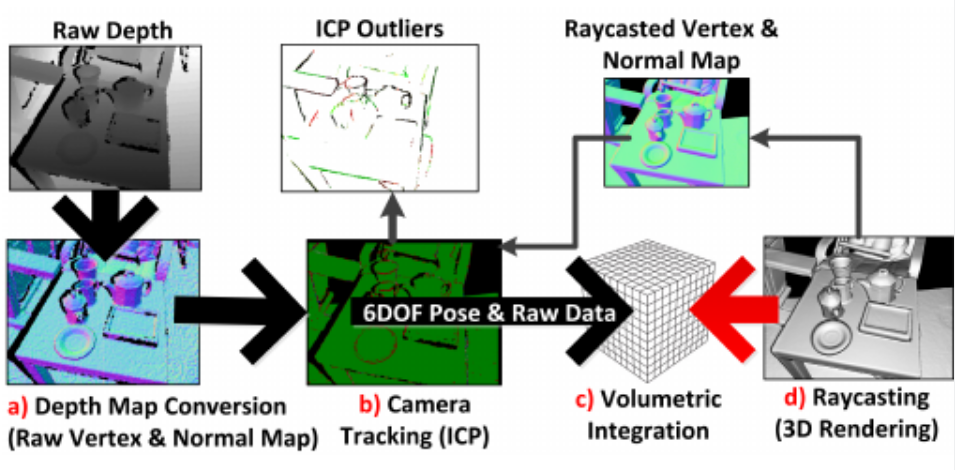
\includegraphics[width=0.66\textwidth, frame]{images/kinfu-integration.png}
	\caption{Integration eines Tiefenbilds in \ac{KinFu}. Entnommen aus \cite{izadi2011kinectfusion}}
	\label{fig:kinfu-integration}
\end{figure}

Durch eine schnelle GPU-Implementierung auf Basis von CUDA erreicht \ac{KinFu} dabei eine Integration neuer Tiefenbilder bei 30 Hz, der Bildwiederholfrequenz der Kinect.
Somit ist die zeitliche Differenz zwischen zwei Aufnahmen sehr niedrig.
Es wird davon ausgegangen, dass die Kamera handgeführt (bzw. mit geringer Geschwindigkeit bewegt) wird, daher hält sich auch die räumliche Distanz zwischen einzelnen Frames in Grenzen.
Aufgrund dieser Gegebenheiten reicht bei \ac{KinFu} eine lokale Registrierung aus, es kann also direkt \ac{ICP} verwendet werden.

In \autoref{fig:kinfu-integration} ist der Ablauf der Integration eines neuen Tiefenbilds ins \ac{TSDF} bei \ac{KinFu} dargestellt.
Das Tiefenbild wird zunächst in eine Punktwolke konvertiert.
Diese wird anschließend durch \ac{ICP} registriert, um dann unter Bildung eines Mittelwerts in das \ac{TSDF} integriert zu werden.
Zur Darstellung der Szene wird dieses anschließend mithilfe eines Raycasters gerendert.


% Hier YAK erwähnen und erklären
% YAK evtl. in Implementierung
Es gibt zahlreiche Optimierungen und veränderte Versionen von \ac{KinFu}.
Unter anderem gibt es in der \ac{PCL} eine freie Implementierung \cite{pirovano2012kinfu}.
Eine optimierte Version ist beispielsweise Chisel \cite{klingensmith2015chisel}, wo eine effizientere Voxelstrategie verwendet wird.
Weiterhin ist Chisel eine reine CPU-Implementierung, was die Nutzung auf Mobilgeräten ohne Grafikkarte ermöglicht.

Die in dieser Arbeit verwendete Implementierung ist \ac{YAK}.
\ac{YAK} ist eine auf \ac{ROS} angepasste Version von \ac{KinFu}, um Trajectory Waypoints für die Robotersteuerung zu errechnen \cite{schornak2019yak}.
Die Verwendung von \ac{KinFu} in industriellen Robotikanlagen ist in vielerlei Hinsicht sinnvoll:
\begin{itemize}
\item Objekte können aus mehreren Perspektiven gescannt werden, was eine bessere Darstellung der Szene liefert.
\item Rauschen durch den Bildsensor wird aufgrund der Mittelwertbildung minimiert.
Das Ergebnis ist ein glatteres und realistischeres Modell.
\item Durch die GPU-Implementierung können Tiefenbilder in Echtzeit integriert werden, was insbesondere bei Robotikanwendungen ein großer Vorteil ist.
\item Ein häufig in der Bildverarbeitung auftretendes Problem sind reflektierende bzw. spiegelnde Oberflächen.
Die betroffenen Regionen können oft nur falsch, verzerrt oder gar nicht modelliert werden.
Da hier eine Aufnahme aus mehreren Perspektiven möglich ist, können derartige Fehler weitestgehend vermieden werden. In \autoref{fig:yak-reflecting-model} ist dies an einem Beispiel besonders gut sichtbar.
\end{itemize}

\begin{figure}[ht]
	\centering
	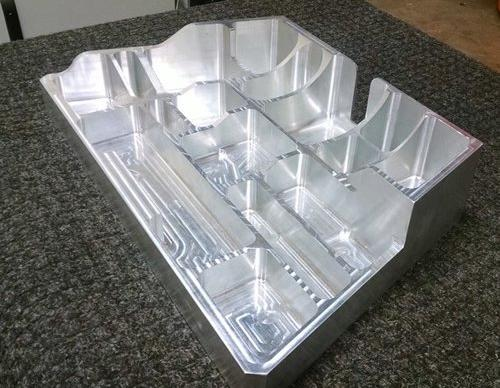
\includegraphics[width=0.4\textwidth]{images/yak-reflecting-scene.jpg}
	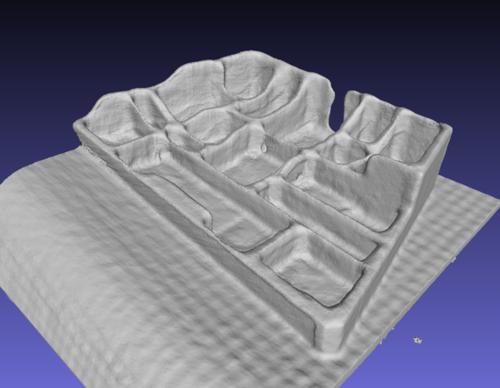
\includegraphics[width=0.4\textwidth]{images/yak-reflecting-reconstruction.png}
	\caption{Szene und Rekonstruktion eines reflektierenden Objekts durch \ac{YAK}. Entnommen aus \cite{schornak2019yak}}
	\label{fig:yak-reflecting-model}
\end{figure}


\subsection{Globale Registrierung}
\label{subsec:global-registration}

Bei der globalen Registrierung müssen sich die beiden Punktwolken nicht nahe der endgültigen Ausrichtung befinden - Translation und Rotation können beliebig sein.
Ein Nachteil ist jedoch, dass die globale Registrierung oft nur eine Grobregistrierung bietet, also keine optimalen Ergebnisse liefert.
Aus diesem Grund bietet es sich meist an, anschließend noch eine lokale Registrierung zur Verbesserung der Ergebnisse durchzuführen.

Zur globalen Registrierung von Punktwolken existieren verschiedene Ansätze \cite{chaudhury2015global, zhou2016fast, rusu2009fast}.
Die in dieser Arbeit verwendete Methode ist Super4PCS \cite{mellado2014super4pcs}, eine optimierte Version von \ac{4PCS} \cite{aiger2008fpcs}.
Dieser Ansatz wird verwendet, da die vorhandene Implementierung \ac{OpenGR} \cite{mellado2018opengr} über einen Wrapper bereits zur \ac{PCL} kompatibel ist.

%TODO 4PCS Funktionsweise erklären


\section{Segmentierung}
\label{sec:segmentation}

Ziel der Segmentierung ist es, zusammengehörende Bildregionen zu identifizieren und durch Zuweisung verschiedener Klassen voneinander zu trennen.
Dies ist, insbesondere in der 2D-Bildverarbeitung, ein altes Problem, für das es viele verschiedene Lösungsansätze gibt.
Auch im dreidimensionalen Raum ist eine Segmentierung häufig notwendig.
Häufig gibt es dabei nicht eine beste Methode - die Objektart, -größe, -form und viele weitere Faktoren beeinflussen die Wahl eines geeigneten Ansatzes.

Die Forschung ist in diesem Bereich weiterhin sehr aktuell:
Beispielsweise zeigen \citeauthor{uckermann2012real} einen Versuch, in Echtzeit und ohne vorher bekannte Objekte zu segmentieren \cite{uckermann2012real}.
Eine Übersicht bieten \citeauthor{nguyen20133d}, die verschiedene Varianten vergleichen und die Vor- und Nachteile diskutieren \cite{nguyen20133d}.
In den letzten Jahren findet auch verstärkt Forschung zur Segmentierung mithilfe von Neuronalen Netzen statt \cite{te2018rgcnn}.

% Segmentierung auf Meshes
Survey \cite{shamir2008survey}, SDF \cite{shapira2008consistent}


\section{Triangulierung}
\label{sec:triangulation}


\subsection{Marching Cubes}
\label{subsec:marching-cubes}
%TODO
Marching Cubes \cite{lorensen1987marching} \autoref{alg:marching-cubes}

\begin{algorithm}[ht]
\caption{Marching Cubes}
\label{alg:marching-cubes}
\begin{algorithmic}
\Function{marchingCubes}{}
	\State $vertexList \gets \emptyset$
	\Comment{The list of output triangles}
	\State $V \gets Voxels$
	\ForAll{$v \in V$}
		\State $index \gets$ \Call{calculateIndex}{v}
		\State $edgeList \gets edgeTable[index]$
		\ForAll{$edge \in edgeList$}
			\State $vertex \gets$ \Call{interpolate}{$edge[0], edge[1]$}
			\Comment{interpolate corners}
			\State \Call{$vertexList$.add}{$vertex$}
		\EndFor
	\EndFor
\EndFunction
\Function{calculateIndex}{$voxel$}
	\State $voxelIndex \gets 0$
	\For{$cornerIndex \in [0..8]$}
		\If{$voxel[cornerIndex] < isolevel$}
		\Comment{corner inside isosurface}
			\State $voxelIndex\ |=\ 1 << cornerIndex$
			\Comment{Set the i-th bit of the index}
		\EndIf
	\EndFor
	\State \Return{$voxelIndex$}
\EndFunction
\end{algorithmic}
\end{algorithm}


\subsection{Poisson}
\label{subsec:poisson}

%TODO
Poisson \cite{kazhdan2006poisson}


\subsection{Weitere Ansätze}
\label{subsec:triangulation-others}
%TODO Ball Pivot, Greedy Triangulation, (Delaunay?)
Greedy Projection \cite{Marton09ICRA},
Ball Pivoting \cite{bernardini1999ball}
